La cosmologia è quella parte della fisica che si occupa di studiare l'origine e l'evoluzione dell'universo, costruendo modelli basati sulla Relatività Generale, assieme alla fisica quantistica, alla fisica delle particelle e molte altre parti della fisica. Tutti questi devono, però, rendere conto agli osservabili cosmologici, ovvero, alle strutture a larga scala, come galassie, radiazione e vuoti (considerandone le proprietà chimiche, cinematiche e le radiative a tutte le lunghezze d'onda), che permetteranno di confermare le predizioni fatte o suggerire delle correzioni.
\section{Principi Cosmologici ed Espansione dell'universo}\label{sec:principi-espansione}
\subsection{Principi Cosmologici}\label{sec:principi-cosmologici}

Tutti i modelli cosmologici proposti devono tenere conto di quelli che sono i \emph{Principi Cosmologici}:
\begin{description}
    \item[omogeneità dell'universo,]cioè in ogni punto il cosmo appaia lo stesso;
    \item[isotropia dell'universo,]ovvero che ci si possa spostare in ogni direzione senza differenze.
\end{description}
Queste due condizioni comportano che non esista un sistema di riferimento o una direzione privilegiata e quindi che un osservatore sia in grado di misurare le stesse caratteristiche medie indipendentemente dalla sua posizione o dal suo movimento. Si arriva quindi a ipotizzare che non esista alcun centro dell'universo, né alcun limite ad esso. Queste ipotesi sono rimaste arbitrarie fino a poco tempo fa, quando si sono avute le prime conferme sperimentali, grazie al \emph{Casmic Microwave Background} (CMB) e alla distribuzione degli ammassi di galassie, come si osserva in figura~\ref{fig:APM}.
\begin{figure}
    \centering
    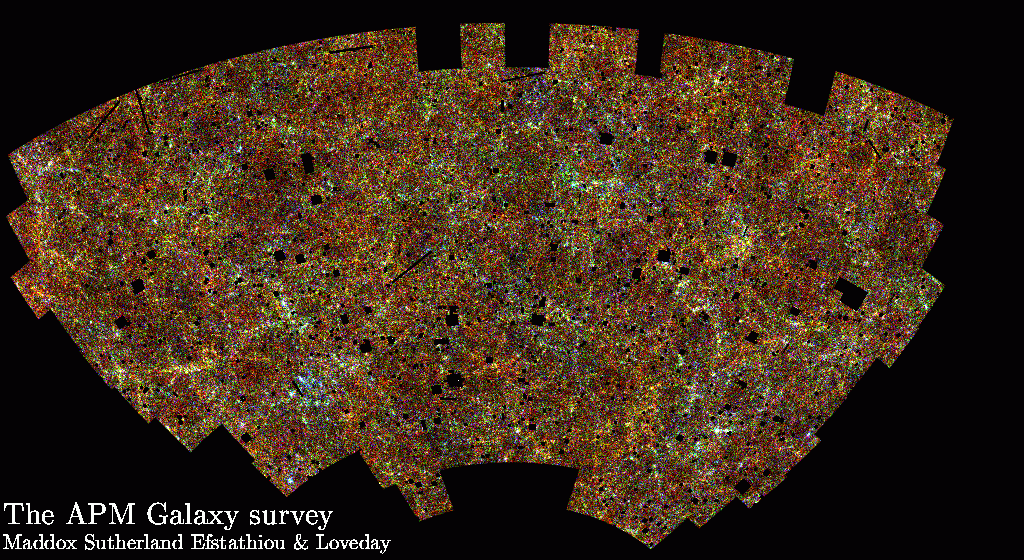
\includegraphics[width=0.45\textwidth]{immagini/APM.png}
    \caption{La figura mostra la distribuzione di ammassi di Galassie nel cielo osservabile, si nota come la distribuzione risulta pressoché uniforme.}\label{fig:APM}
\end{figure}
\subsection{Espansione dell'universo e Red-Shift}\label{sec:espansione}

Nel 1929 Edwin Hubble si rese conto che le linee spettrali delle galassie venivano spostate verso il rosso proporzionalmente alla loro distanza, ne dedusse che questa variazione cromatica fosse dovuta alla  presenza di un effetto Doppler e che di conseguenza le galassie si stessero allontanando con una certa velocità da un osservatore. Le galassie sembrano quindi recedere con una velocità proporzionale con la loro distanza.

\begin{figure}
    \centering
    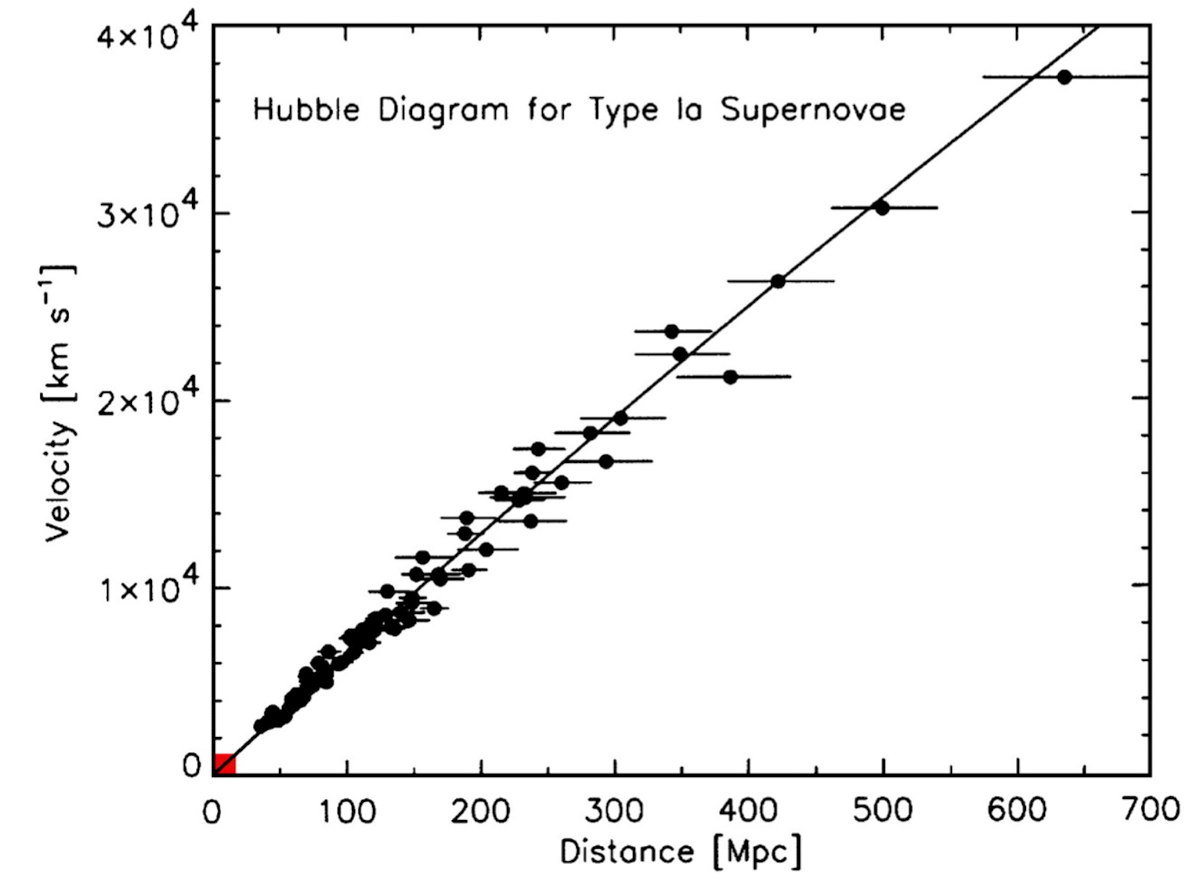
\includegraphics[width=0.4\textwidth]{immagini/redshift.png}
    \caption{La mostra la relazione tra velocità di allontanamento in funzione della distanza, questa è stata stimata misurando la luminosità di supernove di tipo I.a.}\label{fig:redshift}
\end{figure}

Secondo i principi cosmologici l'osservatore non può occupare un posto privilegiato nell'universo, per cui le galassie devono allontanarsi l'una dall'altra, con velocità proporzionale alla distanza tra di loro. Questa dipendenza è ben rappresentata dalla relazione di Hubble:
\begin{equation}\label{eq:hubble}
    v = H_0 D
\end{equation}
dove $H_0 \simeq \SI{73}{km.s^{-1}.Mpc^{-1}}$ ($s^{-1}$)è la costante di Hubble odierna. Il valore esatto di questa costante è ancora dibattuto soprattutto a causa della complessità nella misurazione delle distanze esatte tra le varie galassie e nel distinguere la velocità degli ammassi, rispetto alle velocità delle galassie interne all'ammasso.

Se, quindi, le galassie si stanno allontanando l'una dall'altra senza che esista un centro dell'espansione allora ad espandersi deve essere lo spazio-tempo stesso, il quale trascina con se tutto ciò che è in esso contenuto. Questa è la causa del \emph{red-shift} che osservava Hubble. Se, infatti, è l'universo stesso che si sta espandendo allora la radiazione che lo attraversa si espande insieme a lui e perciò, quando arriva a un osservatore molto distante, sembra spostata verso il rosso. Indicando con $z$ il redshift cosmologico, lo si calcola utilizzando l'equazione~\eqref{eq:redshift}:
\begin{equation}\label{eq:redshift}
    z = \frac{\lambda_\textup{obs} - \lambda_\textup{em}}{\lambda_\textup{em}}
\end{equation}
dove $\lambda_\textup{em}$ è la lunghezza d'onda emessa, mentre $\lambda_\textup{obs}$ è la lunghezza d'onda osservata e modificata a causa del redshift.

Mettendo insieme l'equazione~\eqref{eq:hubble} di Hubble e l'equazione~\eqref{eq:redshift} si ottiene una equivalenza tra redshift e distanza. Sappiamo infatti che:
\[
    \frac{\lambda_\textup{obs} - \lambda_\textup{em}}{\lambda_\textup{em}} = \frac{v}{c}
\]
dove $c$ è la velocità della luce e $v$ è la velocità di espansione dell'universo, per cui il redshift $z$ non è altro che la velocità di espansione dell'universo in unità di velocità della luce.
\[
    v = \frac{\lambda_\textup{obs} - \lambda_\textup{em}}{\lambda_\textup{em}} c
\]
Per cui inserendo la relazione di Hubble:
\[
    v = H_0 D = c z
\]
\begin{equation}\label{eq:ditanza-redshift}
    D = \frac{c}{H_0}z
\end{equation}

Si noti che non esistono delle condizioni sui valori che $z$ può assumere, si deduce che potenzialmente il redshift può valere anche più di uno, questo vuol dire che lo spazio-tempo si espande più velocemente della luce. La relatività ristretta non vieta questo tipo di cose, poiché essa impone la velocità della luce come limite all'interno di quello che è il nostro universo, ma non da indicazioni su cosa succeda all'universo stesso o al suo esterno.